% !Mode:: "TeX:UTF-8"%確保文檔utf-8編碼
\documentclass{standalone}

\usepackage{tikz}


\usepackage{pgfplots}

\RequirePackage[CJKecglue={\hskip 0pt}]{xeCJK}
\xeCJKsetup{PunctStyle=plain}
\setCJKmainfont[ItalicFont=KaiTi]{Source Han Serif CN}
\setCJKsansfont{Source Han Sans CN}
\setCJKmonofont{KaiTi}

\usetikzlibrary{intersections,calc,positioning}

\begin{document}

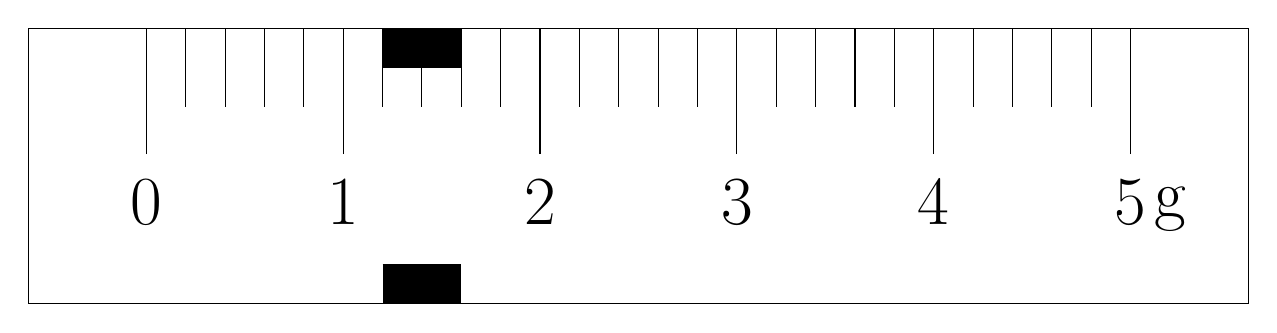
\begin{tikzpicture}[xscale=0.5]

%主线轴
\def\startx{0}
\def\endx{25}
\pgfmathsetmacro{\stepx}{\startx+1}
\pgfmathsetmacro{\stepxfive}{\startx+5}
\pgfmathsetmacro{\stepxten}{\startx+10}

\coordinate (startpoint) at (\startx,0) ;
\coordinate (endpoint) at (\endx,0) ;
\draw [](startpoint) -- (endpoint);

\draw ($(startpoint) + (-3,-3.5)$) rectangle ($(endpoint) + (3,0)$);

%细小刻度
\foreach \x in {\startx,\stepx,...,\endx}
  \draw [](\x,0) -- (\x,-1);   

%5分之一刻度
%\foreach \y in {\startx,\stepxfive,...,\endx}
%  \draw [] (\y,-1.6) -- (\y,0);


%10分之一刻度
\foreach \i in {\startx,\stepxfive,...,\endx}
  \draw [] (\i,-1.6) -- (\i,0)
  node[below=1.8cm] {\Huge \pgfmathprint{int(\i/5)}};

%unit
\node at ($(endpoint) +(1,-2.3)$) {\Huge  g};


%额外的修改
\draw[line width =0.5cm,yshift=-0.25cm] (6,0)-- (8,0);
\begin{scope}[yshift=-3cm]
\draw[line width =0.5cm,yshift=-0.25cm] (6,0)-- (8,0);
\end{scope}



\end{tikzpicture}


\end{document}